% One-slide highlight talk (16:9). Compile in results/ so the figure resolves.
\documentclass[aspectratio=169,10pt]{beamer}

\usepackage[T1]{fontenc}
\usepackage{lmodern}
\usepackage{graphicx}
\usepackage{xcolor}

\setbeamertemplate{navigation symbols}{}
\setbeamertemplate{itemize items}{\textbullet}
\definecolor{accent}{HTML}{1F6F78}
\setbeamercolor{itemize item}{fg=accent}
\setbeamercolor{itemize subitem}{fg=accent}
\hypersetup{colorlinks=true,urlcolor=accent}

% Compact itemize: small font, tight spacing, no bullet over-indent.
\newenvironment{tight}
  {\begin{itemize}\fontsize{7}{7.0}\selectfont
     \setlength{\itemsep}{0pt}\setlength{\parskip}{0pt}\setlength{\topsep}{0pt}
     \setlength{\leftmargini}{1.05em}}
  {\end{itemize}}

% Coloured section header with an underline rule.
\newcommand{\sect}[1]{%
  \vspace{1pt}{\color{accent}\bfseries\footnotesize #1}\par
  \vspace{-0.45em}{\color{accent}\rule{\linewidth}{0.6pt}}\par\vspace{0pt}}

\newcommand{\pc}{\textperiodcentered}

\begin{document}
\begin{frame}[t]

% ---- header banner ----
\noindent\colorbox{accent}{%
  \parbox[t]{\dimexpr\textwidth-2\fboxsep\relax}{\vspace{1pt}%
    {\color{white}\bfseries\large Remote work, team velocity \& long-term capability}\\[0.5pt]
    {\color{white!85!accent}\footnotesize An agent-based model of a software-development team
     \hfill Mi\l osz Lewandowski}\vspace{1pt}}}
\par\vspace{1.5pt}
{\scriptsize Code: \href{https://github.com/milolew/sprint-velocity-simulation}{github.com/milolew/sprint-velocity-simulation}
 \quad\textbullet\quad Live demo: \href{https://sprint-velocity-simulation-6oaiwsd3eqgf6r3qwfapkz.streamlit.app/}{interactive Streamlit app}}
\par\vspace{1pt}

% ---- two columns ----
\begin{columns}[T]
\begin{column}{0.54\textwidth}

  \sect{1\,\pc\, Goal}
  \begin{tight}
    \item How does the share of \textbf{remote work} affect a software team's
          \textbf{output} and \textbf{long-term capability}?
    \item \textbf{Decision support}: not one average effect, but
          \emph{under which conditions} remote work is cheap vs costly.
  \end{tight}

  \sect{2\,\pc\, Agents \& environment}
  \begin{tight}
    \item \textbf{10 developer agents}, each a per-tick state machine:
          idle $\to$ working $\to$ blocked $\to$ helping.
    \item \textbf{Environment}: a backlog of story-point tasks; time in
          15-min ticks, 10-day sprints, $\sim$1-year horizon.
    \item Each morning each dev is office/home w.p.\ \texttt{remote\_share}
          --- the one policy lever.
    \item \textbf{Help channel}: office$\leftrightarrow$office is fast/synchronous
          (teaches more); any-home help is slow/asynchronous.
  \end{tight}

  \sect{3\,\pc\, What happens \pc\ what I added}
  \begin{tight}
    \item Base model: \emph{one sprint}, fixed skill. \textbf{My extension}: a full
          \textbf{year} with \textbf{learning-by-doing} \& \textbf{turnover}
          (juniors replace leavers and must learn).
    \item \texttt{remote\_share} now also drives \textbf{skill growth}
          (remote $\Rightarrow$ more async help $\Rightarrow$ slower ramp) and \textbf{retention}.
  \end{tight}

\end{column}
\begin{column}{0.44\textwidth}

  \centering
  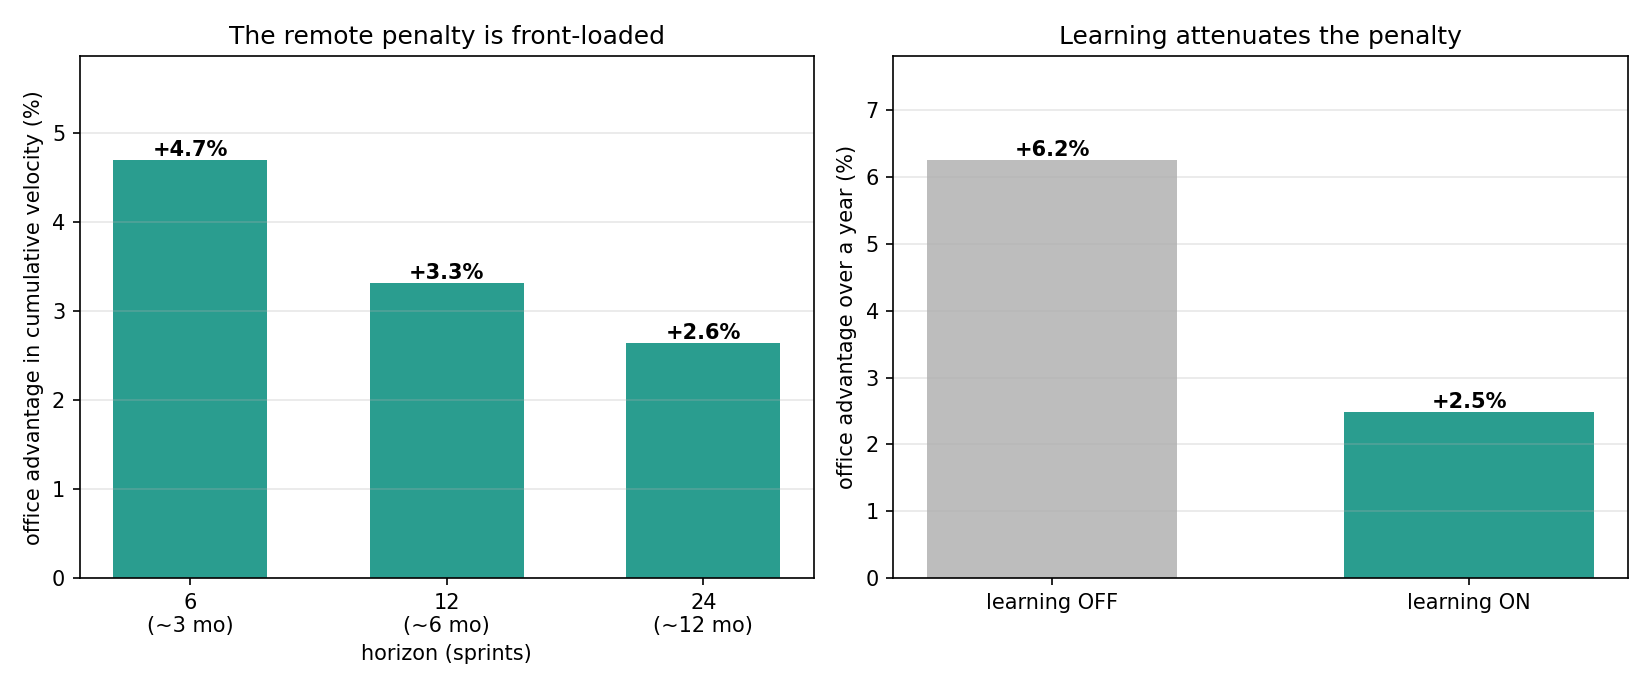
\includegraphics[width=0.70\linewidth]{partb_penalty.png}\\[1pt]
  {\scriptsize The office advantage shrinks over the year (left); turning learning
   on more than halves it (right).}

  \raggedright
  \sect{4\,\pc\, Key findings}
  \begin{tight}
    \item Sprint penalty scales with how often help is needed:
          $-3.6\%$ (skilled) to $-13.2\%$ (block-prone).
    \item Over a year the gap is only $\sim\!2.5\text{--}2.8\%$ and
          \textbf{front-loaded, not compounding} --- largest while the team is
          junior, then learning erases it (\emph{reverses the prior}).
    \item Biggest decision-relevant effect: the \textbf{spread} of yearly
          output ($\sim\!3\times$), not the mean.
    \item $\Rightarrow$ \textbf{Cheap for mature, stable teams; costly for
          junior-heavy, high-churn} ones.
  \end{tight}

\end{column}
\end{columns}

\end{frame}
\end{document}
